\subsection{Representación Gráfica de Señales Sinusoidales}

En esta sección se considera la señal de tiempo discreto $y(t) = sin(t/6)$, y se realizan dos muestreos, utilizando el comando \texttt{stem} de MATLAB, en una ventana de una ventana de 60 segundos. El primero de ellos toma 30 muestras y el segundo 6 muestras. Además se grafica dicha señal utilizando el comando \texttt{plot}. Los resultados obtenidos en el proceso se reflejan en la figura \ref{plot_stem}.

\begin{figure}[H]
    \centering
    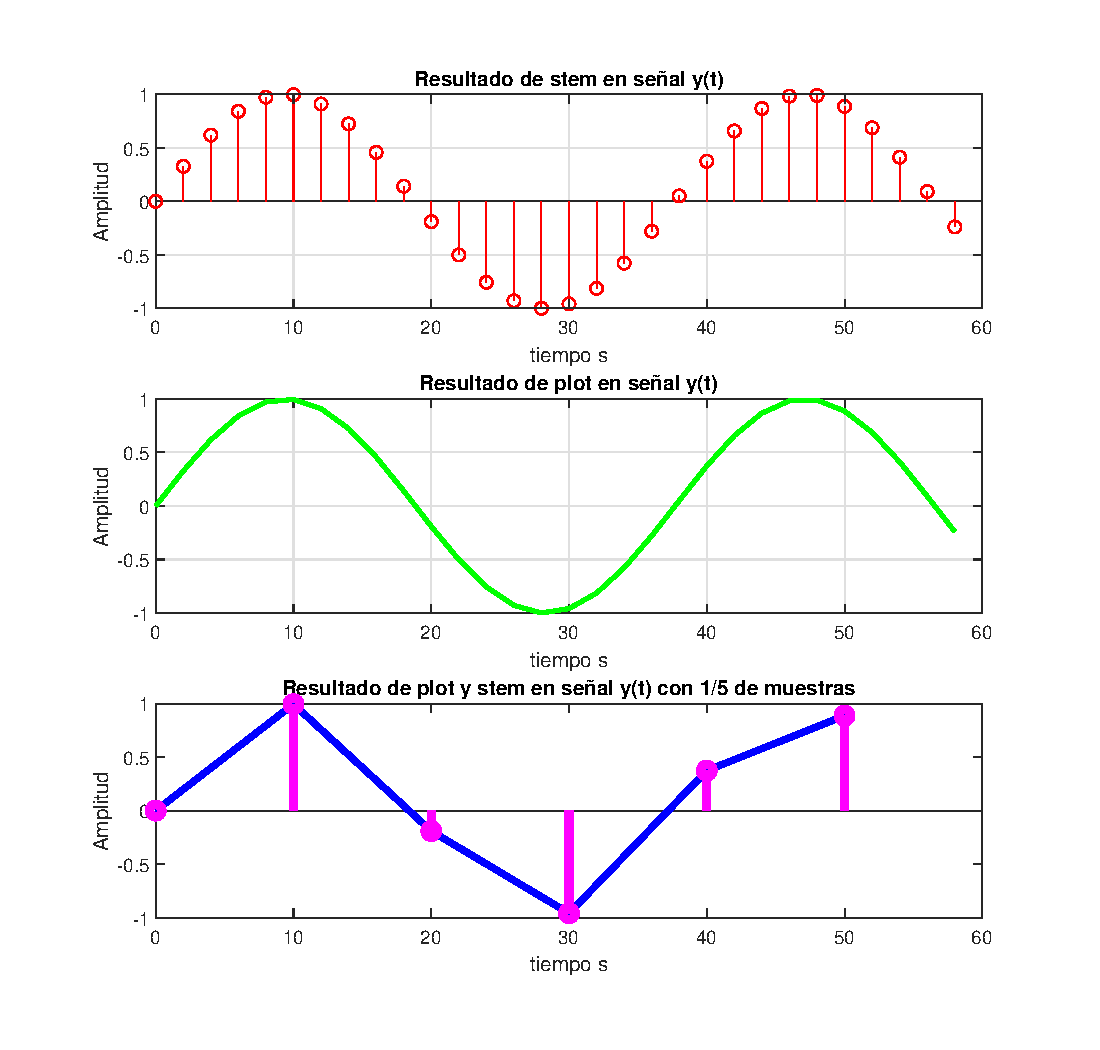
\includegraphics[scale = 0.8]{Imagenes/representacion_sennales.eps}
    \caption{Resultado de  comandos \textit{plot} y \textit{stem} aplicados a la señal $sin(t/6)$ }
    \label{plot_stem}
\end{figure}




\begin{enumerate}

    \item La figura  \ref{plot_stem} presenta tres gráficos, el primero muestra el resultado obtenido al aplicar el comando \texttt{stem} a la señal $y(t)$ considerando 30 muestras; el segundo muestra el resultado de graficar la señal $y(t)$ utilizando el comando \texttt{plot};  el tercero muestra el resultado de aplicar el comando \texttt{stem} a la señal $y(t)$ considerando 6 muestras además de graficarla utilizando el comando \texttt{plot}.
    
    \item Se puede notar que en los gráficos en los que se utiliza el comando \texttt{stem},se logra una clara representación de tiempo discreto de la señal, generando un punto en los instantes en que se toma la muestra de esta, mientras que cuando se utiliza el comando \texttt{plot}, lo que se obtiene es una gráfica que simula una señal de tiempo continuo a pesar de que la señal original corresponde a tiempo discreto. Esto se ve claramente en el tercer gráfico de la figura \ref{plot_stem}, en donde a pesar que se redujo el número de muestras tomadas, por lo que el espacio entre ellas es mayor, el resultado que se tiene  con el comando \texttt{plot} es una señal continua  que pierde la forma original de la señal, mientras que con el comando \texttt{stem}, aún se puede recuperar parte de la información se la señal $y(t)$ muestreada.
    
    \item Cuando se obtienen 30 muestras de la señal, el resultado obtenido es una señal claramente discreta que preserva la forma de la señal original $y(t)$, mientras que en el caso en que se reduce el numero de muestras en cinco veces, si bien la forma no es tan explicita respecto a la señal original, el número de muestras es suficiente para cumplir el criterio de Nyquist por lo que de todas formas se puede recuperar la señal $y(t)$. Se puede concluir que tomar 30 muestras de la señal no es estrictamente necesario para la señal que se está trabajando.
    
    \item El intervalo de $[0:59]$, corresponde a una ventana de 60 unidades de tiempo. No se especifica sobre que unidad puede ser. %durante las cuales se puede analizar la señal $y(t)$, se puede interpretar como una ventana de 60 segundos.
    
    %5
    \item 
    
    %Ambas señales tienen una duración de 60s, asumiendo que $t$ corresponde un intervalo de 1 minuto. Lo que cambia las señales discretas es el periodo de muestreo.
    
    No tiene sentido hablar de duración en segundos y frecuencia en Hz si no se conoce el periodo de muestreo.
    
    Siendo la frecuencia de muestro $f_s$, la duración en segundos de la primera sinusoide correspondería a:
    $$ \text{Duración} = \dfrac{60}{f_s}$$
    
    La frecuencia de la sinusoide discreta corresponde a la frecuencia relativa ($f_r$). A partir de la expresión para la frecuencia relativa se concluye que:
    $$ f_r = \dfrac{f}{f_s} \Rightarrow f = f_r\cdot f_s$$
    Por lo tanto para la primera sinusoide la frecuencia en Hz corresponde a:
    $$f = \dfrac{1}{2\pi}\cdot \dfrac{1}{6} f_s$$.
    
    La duración y frecuencia de la segunda sinusoide coincidiría con la primera, asumiendo una nueva frecuencia de muestreo acorde a un downsampling con un factor de 5.
    %No tiene sentido hablar de duración en segundos y Hz de una señal digital sin antes pasarla por DAC y un filtro. Para contestar la duración en tiempo y Hz se asumirá un retentor de orden cero para pasar de la discreta a la señal de tiempo continuo.
    
    %De esta ambas señales duran 60s y no serían periódicas.
    
    %No se cumple la periodicidad por no interpolar correctamente (el teorema del muestreo implica reconstrucción perfecta interpolando con funciones $ sinc $ ).
    

%\begin{table}[htbp]
%\begin{center}
%%\begin{tabular}{|l|l|l|}
%%%\hline
%%Señal  & Duracion [s]  & frecuencia [Hz] \\
%\hline \hline

%Señal muestreada con $n = 30$   &  \hspace{0.7cm}    2   & $\frac{6}{10}$\\ \hline

%Señal muestreada con $n = \frac{30}{5}$ & \hspace{0.7cm}  10  & $\frac{1}{10}$ \\ \hline

%\end{tabular}
%\caption{Duración en s y  frecuencia en Hz de las señales obtenidas.}
%\label{duracion_frec}
%\end{center}
%\end{table}

    
    \item El comando \texttt{stairs} asi como el comando \texttt{stem} o el comando \texttt{plot}, genera una figura en MATLAB que grafica una interpretación de la señal que se le ingresa como parámetro. Este comando en particular, a diferencia de \texttt{plot}, genera puntos cada vez que lee una muestra del vector/señal, e interpola generando puntos que conservan el valor de la última muestra hasta que lee una nueva muestra y repite el proceso, es decir, este comando se comporta como un circuito retentor de orden cero, o como un flip flop, ya que toma un valor y lo mantiene constante hasta tomar otro nuevo.
    
    En la figura \ref{stairs} se muestra una comparativa entre el uso del comando \texttt{plot} y el comando \texttt{stairs()}.
    
    \begin{figure}[H]
        \centering
        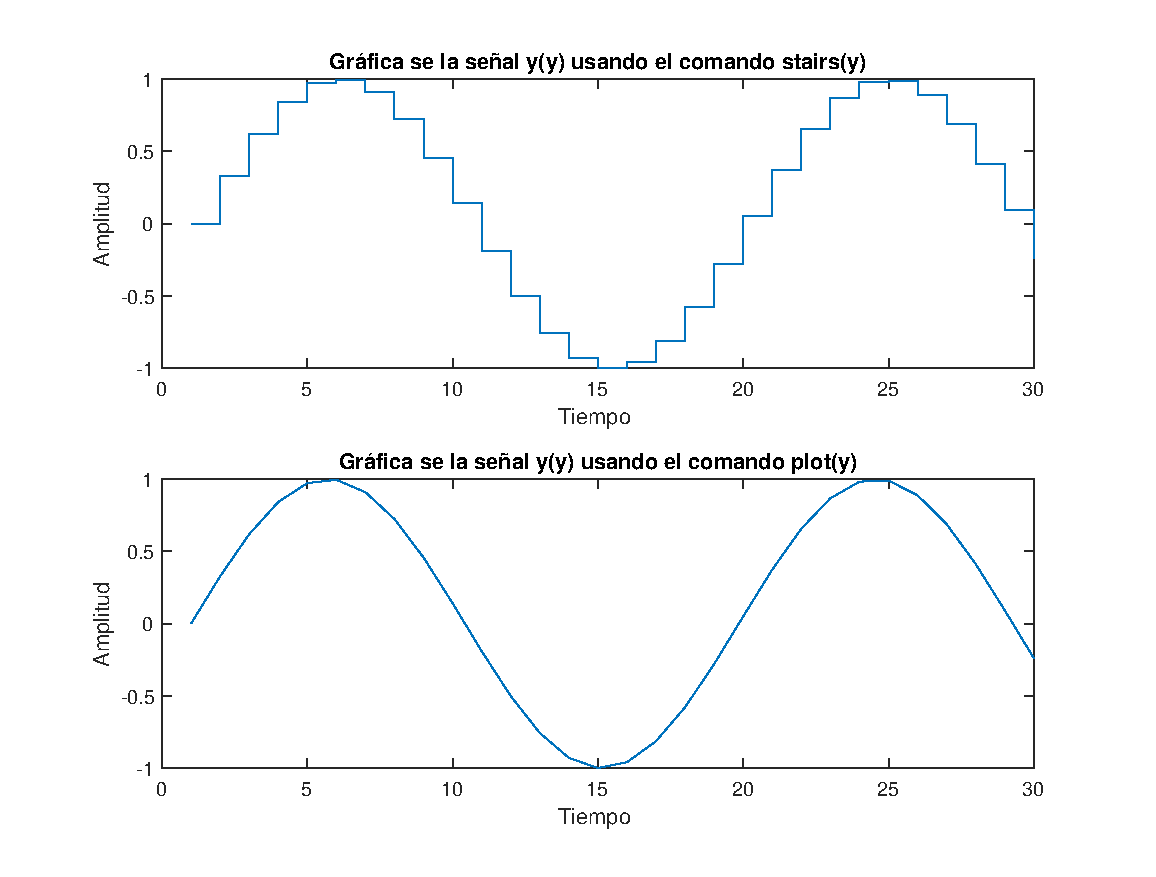
\includegraphics[scale = 0.6]{Imagenes/stairs.eps}
        \caption{Gráfica de la señal y(t) usando los comandos \texttt{plot} y el comando \texttt{stairs()}}
        \label{stairs}
    \end{figure}
    
    
    
    
    
\end{enumerate}

